[96~v\textsuperscript{o}] altitudinem siphonis\protect\index{Sachverzeichnis}{sipho} ultra vas, \edtext{non esse minorem}{\lemma{vas,}\Afootnote{ \textit{ (1) }\ majorem \textit{ (2) }\ non esse minorem \textit{ L}}} quam est altitudo descensus in vase, alioqui \textit{D} lateribus  vasis impingeret; ac denique circumspiciendum est de exacta quadam \edtext{effluxus}{\lemma{}\Afootnote{quadam  \textbar\ guttarum \textit{ gestr.}\ \textbar\ effluxus \textit{ L}}} mensuratione. Ex quibus haec mihi maxime placuit; applicetur instrumentum quale passibus numerandis adhibetur, in \edtext{latus unum rotae primae liquor extillans effluensve}{\lemma{in}\Afootnote{ \textit{ (1) }\ hoc \textit{ (2) }\ hujus rotam\protect\index{Sachverzeichnis}{rota|textit} \textit{ (3) }\ rotae\protect\index{Sachverzeichnis}{rota|textit} primae latus  unum desi \textit{ (4) }\ latus [...] effluensve \textit{ L}}} guttae extillantes, incidant, ac proinde Rotam\protect\index{Sachverzeichnis}{rota} circumagant, rotae\protect\index{Sachverzeichnis}{rota} conversiones ab instrumento numerabuntur\edtext{. Ponamus}{\lemma{numerabuntur}\Afootnote{ \textit{ (1) }\ , et apparebit praeterea \textit{ (2) }\ . Ponamus \textit{ L}}} rotam\protect\index{Sachverzeichnis}{rota} semel circumagi uno minuto secundo (quod  utique procurari non difficile est), \edtext{et}{\lemma{est),}\Afootnote{ \textit{ (1) }\ ponamus \textit{ (2) }\ et \textit{ L}}} rotam\protect\index{Sachverzeichnis}{rota} ipsam  rursus in 60 dentibus\protect\index{Sachverzeichnis}{dens} \edtext{distingui}{\lemma{dentibus}\Afootnote{ \textit{ (1) }\ esse \textit{ (2) }\ distingui \textit{ L}}}; manifestum est ad tertia usque minuta procedi posse quorum 216000 horam\footnote{\textit{Nebenrechnung}:\\
$\protect\begin{array}{l} ~~6000\\~~6\\\overline{~36000}\\\protect\raisebox{0.5ex}{3}~6~~~\\\overline{216000}\protect\end{array}$
} \edtext{componunt.}{\lemma{}\Afootnote{componunt.  \textbar\ Et \textit{ (1) }\ fortasse in mari usus \textit{ (2) }\ cogitandum est an non \textit{(a)}\ hujus instrumenti usus in mari sit ipso pendulo\protect\index{Sachverzeichnis}{pendulum|textit} \textit{(b)}\ hoc instrumentum sit ad maris \textit{(c)}\ hujus instrumenti usus possit esse in mari. Magna dubitatio est, an non pendula ipsa   \textbar\ in longinquis itineribus \textit{ erg.}\ \textbar\  pro aeris conditione varient; rationis enim est tardiores esse vibrationes in  aere crassiore; at aeris variatio Mercurium, quem ego consultissime adhiberi puto nec dilatabit magis nec rarefiet,  nec premet certe, ut in Baroscopio, quia premere potest  ab omni parte. Quod pertinet ad perturbationem  motus per jactationes navis, primum ut pendulum, ita et hoc instrumentum suspendi potest,  \textit{(aa)}\ penduli\protect\index{Sachverzeichnis}{pendulum|textit} vibratio \textit{(bb)}\ deinde si pendulum jactatur. \textit{ gestr.}\ \textbar\ Utile \textit{ L}}} Utile est autem altitudinem \textit{EC} seu differentiam crurum esse magnam, ita enim fortius premetur  citiusque effluet liquor. Et Mercurius\protect\index{Sachverzeichnis}{mercurius} \edtext{inter caeteros}{\lemma{}\Afootnote{inter caeteros \textit{ erg.} \textit{ L}}} commoditatem habet, quod non gelatur, non facile consumitur, fortius cadit fluitque. \pend \newpage
  \noindent\textit{Nicht zuzuordnende Zeichnungen in der rechten Spalte}:\\
  \begin{center}
%Zeitz auskommentiert  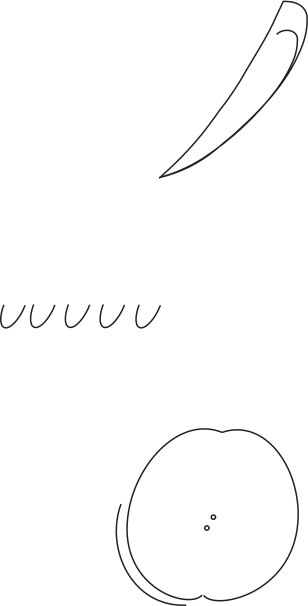
\includegraphics[width=0.2\textwidth]{images/37_3_96r345.pdf}
  \hspace{20mm}
  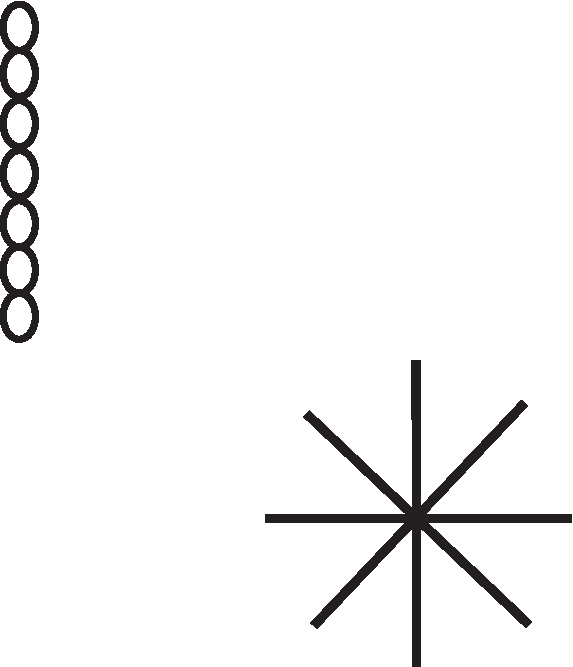
\includegraphics[width=0.2\textwidth]{images/37_3_96v1.pdf}
  \end{center}
  \vspace{1.0ex}
  %\includegraphics[width=0.4\textwidth]{images/37_3_96r_calc5.pdf}
  \textit{Nicht zuzuordnende Rechnungen in der rechten Spalte}:\\
  \vspace{2.0ex}
  \begin{tabular}{rcrcr}
  16 & \textendash & 26 & \textendash & 14 \\
  8 & & & & 7 \\
  4 & & 13 & & 7 \\
  & & & & 13
  \end{tabular}\\
  \rule{38mm}{0.4pt}\\
  \rule{34mm}{0pt}91 \hspace{6mm}
  $\protect\begin{array}{l} \cancel{1}3\\\cancel{9}\cancel{1} \hspace{5.5pt}f\hspace{5.5pt}22\protect\displaystyle\protect\frac{3}{4}\\\cancel{4}\cancel{4}\protect\end{array}$